\section{Database}
Il database utilizzato per il progetto è PostgreSQL. E' stato progettato seguendo questo modello ER:

\begin{figure}[H]
    \centering
    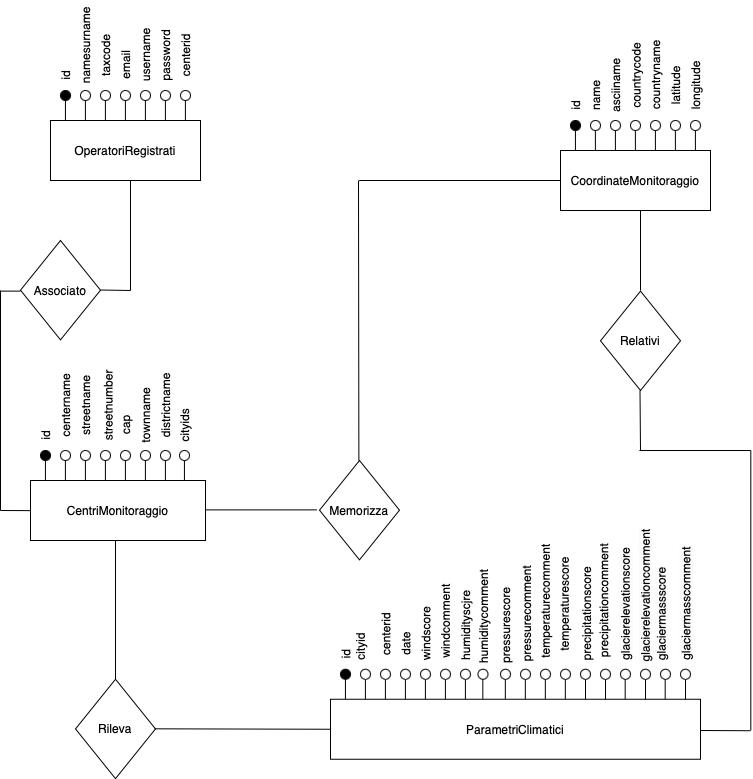
\includegraphics[width=0.8\textwidth]{img/Schema_ER.jpg}
    \caption{Modello ER del database}
    \label{fig:ER}
\end{figure}

\subsection{Schemo Logico}
Il database è composto da 4 tabelle:
\begin{itemize}
    \item \textbf{CoordinateMonitoraggio}(\underline{id}, name, asciiname, countrycode, countryname, latitude, longitude);
    \item \textbf{CentriMonitoraggio}(\underline{id}, centername, streetname, streetnumber, cap, townname, districtname, cityids\textsuperscript{CoordinateMonitoraggio});
    \item \textbf{OperatoriRegistrati}(\underline{id}, namesurname, taxcode, email, username, password, centerid\textsuperscript{CentriMonitoraggio});
    \item \textbf{ParametriClimatici}(\underline{id}, cityid\textsuperscript{CoordinateMonitoraggio}, centerid\textsuperscript{CentriMonitoraggio}, date, windscore, windcomment, humidityscore, humiditycomment, pressurescore, pressurecomment, temperaturescore, temperaturecomment, precipitationscore, precipitationcomment, glacialelevationscore, glacialelevationcomment, glaciamassscore, glacialmasscomment).
\end{itemize}

\subsection{Progettazione}
Qui verranno elencati gli script SQL per la creazione delle tabelle.

\subsubsection{Creazione Database}
\begin{lstlisting}[language=SQL]
CREATE DATABASE climatemonitoring;
\end{lstlisting}

\subsubsection{Creazione tabella coordinatemonitoraggio}
\begin{lstlisting}[language=SQL]
    CREATE TABLE IF NOT EXISTS coordinatemonitoraggio (
    id SERIAL PRIMARY KEY,
    name VARCHAR(100) NOT NULL,
    asciiname VARCHAR(100) NOT NULL,
    countrycode CHAR(2) NOT NULL,
    countryname VARCHAR(100) NOT NULL,
    latitude DECIMAL(9, 6) NOT NULL, 
    longitude DECIMAL(9, 6) NOT NULL);
\end{lstlisting}

\subsubsection{Creazione tabella centrimonitoraggio}
\begin{lstlisting}[language=SQL]
    CREATE TABLE IF NOT EXISTS centrimonitoraggio (
    id SERIAL PRIMARY KEY,
    centername VARCHAR(100) NOT NULL,
    streetname VARCHAR(100) NOT NULL,
    streetnumber VARCHAR(10) NOT NULL,
    cap VARCHAR(10) NOT NULL,
    townname VARCHAR(100) NOT NULL, 
    districtname VARCHAR(100) NOT NULL,
    cityids INTEGER[]);
\end{lstlisting}

\subsubsection{Creazione tabella operatoriregistrati}
\begin{lstlisting}[language=SQL]
    CREATE TABLE IF NOT EXISTS operatoriregistrati (
    id SERIAL PRIMARY KEY, 
    namesurname VARCHAR(200) NOT NULL, 
    taxcode VARCHAR(16) NOT NULL UNIQUE, 
    email VARCHAR(100) NOT NULL UNIQUE,
    username VARCHAR(50) NOT NULL UNIQUE,
    password VARCHAR(100) NOT NULL,
    centerid INTEGER, 
    FOREIGN KEY (centerid) REFERENCES centrimonitoraggio(id));
\end{lstlisting}

\subsubsection{Creazione tabella parametriclimatici}
\begin{lstlisting}[language=SQL]
    CREATE TABLE IF NOT EXISTS parametriclimatici (
    id SERIAL PRIMARY KEY, 
    cityid INTEGER NOT NULL, 
    centerid INTEGER NOT NULL, 
    date DATE NOT NULL, 
    windscore INTEGER, 
    windcomment TEXT, 
    humidityscore INTEGER, 
    humiditycomment TEXT, 
    pressurescore INTEGER, 
    pressurecomment TEXT, 
    temperaturescore INTEGER, 
    temperaturecomment TEXT, 
    precipitationscore INTEGER, 
    precipitationcomment TEXT, 
    glacierelevationscore INTEGER, 
    glacierelevationcomment TEXT, 
    glaciermassscore INTEGER, 
    glaciermasscomment TEXT, 
    FOREIGN KEY (cityid) REFERENCES coordinatemonitoraggio(id), 
    FOREIGN KEY (centerid) REFERENCES centrimonitoraggio(id));
\end{lstlisting}

\subsubsection{Opzioni di Sicurezza}

\begin{lstlisting}[language=SQL]
    GRANT SELECT ON coordinatemonitoraggio TO PUBLIC;
\end{lstlisting}

\begin{lstlisting}[language=SQL]
    GRANT SELECT ON parametriclimatici TO PUBLIC;
\end{lstlisting}

Le altre due tabelle non sono state rese pubbliche per motivi di sicurezza.